\section{Results}
\label{sec:results}

\begin{table}[t]
\centering
\caption{Cohen's $d$ for $\Delta\ell_z^*$ across model families ($n{=}10$ clean seeds). Single-seed conditions: percentile bootstrap 95\% CI (10,000 resamples). $^{\dagger}$Multi-seed conditions: mean $\pm$ SD ($n{=}3$ independent runs). All single-seed CIs exclude zero.}
\label{tab:cohens_d}
\footnotesize
\resizebox{\columnwidth}{!}{%
\begin{tabular}{@{}llrrrr@{}}
\toprule
Model & Bench. & $d$ (5\%) [CI] & $d$ (15\%) [CI] & $d$ (25\%) [CI] & $d$ (50\%) [CI] \\
\midrule
Qwen$^{\dagger}$ & MMLU & $-4.15$ [$-9.9$, $-2.7$] & $-5.36$ ($\pm$1.10) & $-7.44$ ($\pm$1.86) & $-5.08$ ($\pm$3.02) \\
Llama$^{\dagger}$ & MMLU & $-2.57$ ($\pm$0.99) & $-2.80$ ($\pm$0.60) & $-2.56$ ($\pm$0.52) & $-2.30$ ($\pm$0.30) \\
Mistral$^{\dagger}$ & MMLU & $-3.83^{*}$ ($\pm$1.42) & $-3.37$ ($\pm$0.68) & --- & $-4.09$ ($\pm$0.53) \\
Qwen$^{\dagger}$ & ARC-C & --- & $+3.16$ [$2.0$, $9.5$] & --- & $+5.30$ [$3.6$, $15.2$] \\
\bottomrule
\multicolumn{6}{@{}l}{\scriptsize $^{\dagger}$Multi-seed conditions: means ($n{=}3$ independent runs) shown as $\pm$SD; remaining conditions are single-seed with bootstrap CIs.} \\
\multicolumn{6}{@{}l}{\scriptsize $^{*}$$n{=}2$ seeds. Per-seed values in Appendix~\ref{app:reproducibility}.}
\end{tabular}}
\end{table}

\subsection{Detection Signal Across Model Families}
\label{sec:detection}

Table~\ref{tab:cohens_d} presents Cohen's $d$ effect sizes for $\ell_z^*$ across three model families and two benchmarks.
All single-seed bootstrap CIs exclude zero, confirming that $\Delta\ell_z^*$ reliably separates contaminated from clean models at both contamination levels.

On MMLU, effect sizes range from $|d|{=}2.30$ (Llama at 50\%) to $|d|{=}7.44$ (Qwen at 25\%), with Qwen at 5\% ($|d|{=}4.15$) confirming detection at the lowest contamination level tested. Llama ($|d|{=}2.57$/$2.80$/$2.56$/$2.30$) and Mistral ($|d|{=}3.83$/$3.37$/$4.09$) show comparable magnitudes.
On ARC-C (295 items), Qwen yields $|d|{=}3.16$ at 15\% and $|d|{=}5.30$ at 50\%, demonstrating that detection remains feasible even on small benchmarks when contamination is sufficiently concentrated.
The positive sign on ARC-C (vs.\ negative on MMLU) reflects a ceiling effect: with 89.7\% baseline accuracy, contamination pushes responses toward over-consistency rather than the unexpected-success pattern seen on MMLU.

Clean-model $\ell_z^*$ baselines diverge substantially: Qwen ${+}8.68$ (over-consistent), Llama ${-}0.14$ (near-expected), Mistral ${+}4.02$ (Appendix~\ref{app:baseline_meaning}); seed sensitivity analysis confirms these reflect systematic misfit rather than seed artifacts (Appendix~\ref{app:seed_sensitivity}), making absolute thresholds uninformative.
The $\Delta\ell_z^*$ design normalizes these divergent baselines (Figure~\ref{fig:heatmap}).

\begin{figure}[t]
  \centering
  
\includegraphics[width=\columnwidth]{fig_heatmap.pdf}
  \caption{Cohen's $|d|$ heatmap (values from Table~\ref{tab:cohens_d}; multi-seed means where available). Blue intensity reflects effect-size magnitude. Grey cells: not tested.}
  \label{fig:heatmap}
\end{figure}

\subsection{Model-Specific $\theta$-Shift Dynamics}
\label{sec:theta_dynamics}

Contamination inflates $\hat{\theta}_{\text{MLE}}$, which ``explains away'' anomalous successes on hard items; we term this \emph{$\theta$-shift absorption}.
$\theta$-shift magnitude is comparable across families ($\Delta\theta{\approx}0.5$), yet fixed-$\theta$ amplification diverges markedly (Table~\ref{tab:theta_fixed}; Figure~\ref{fig:composite}c).

$\theta$-shift absorption is the dominant source of detection variability for high-ability models at high contamination:
(i) fixed-$\theta$ estimation amplifies Qwen's multi-seed $|d|$ by 2.4$\times$ at 50\% ($5.08 \to 12.32$; Table~\ref{tab:theta_fixed}), while Llama shows no amplification ($0.4\times$);
(ii) $\theta$-anchoring reduces Qwen's inter-seed CV from 60\% to 19\%, confirming that training-run variance is driven by $\theta$-shift stochasticity rather than true signal variance;
(iii) the cross-model ranking under free-$\theta$ is seed-dependent at 50\%, making $\theta$-anchoring a necessary condition for reliable detection of high-ability models at high contamination.

ARC-C reverses this pattern: despite 89.7\% baseline accuracy, contamination produces \emph{larger} effect sizes ($|d|{=}3.16$/$5.30$).
This ceiling effect arises because 295 items with high baseline accuracy leave minimal room for $\theta$ inflation; contamination manifests as anomalous successes on the few remaining hard items, producing disproportionately large $\ell_z^*$ shifts.
Detection sensitivity thus depends on the interaction between model ability and benchmark characteristics, suggesting that practitioners should interpret effect sizes relative to the specific model--benchmark pairing rather than applying universal thresholds.

\paragraph{Seen vs.\ unseen decomposition.}
To localize the contamination signal, we recompute $\ell_z^*$ separately on seen and unseen item subsets.
At 15\% contamination, Qwen's seen-item $\ell_z^*$ drops to $+0.67$ while unseen items remain at $+3.91$ (seed 42; clean baseline $+8.68$), confirming that the person-fit signal originates predominantly from memorized items.
This decomposition is unique to $\ell_z^*$ among the statistics we evaluate: neither accuracy $z$-scores nor HT support item-subset analysis.

\paragraph{Fixed-$\theta$ estimation.}
Table~\ref{tab:theta_fixed} compares free- and fixed-$\theta$ Cohen's $d$.
The amplification ratio tracks baseline $|\ell_z^*|$ monotonically: Qwen ($\ell_z^*{=}{+}8.68$) shows $2.4{\times}$ at 50\%, Mistral ($+4.02$) $1.7{\times}$, while Llama ($-0.14$) shows $0.4{\times}$ despite comparable $\theta$-shift ($\Delta\theta{=}0.52$).
Fixed-$\theta$ is thus a targeted remedy for models with substantial baseline misfit, not a universal one.

\begin{table}[t]
\centering
\caption{Free-$\theta$ vs.\ fixed-$\theta$ Cohen's $|d|$ on MMLU. Qwen$^{\S}$: multi-seed mean ($n{=}3$); Llama and Mistral: seed-42 single run. Fixed-$\theta$ anchors $\hat{\theta}$ at the clean-model mean, eliminating $\theta$-shift absorption.}
\label{tab:theta_fixed}
\footnotesize
\resizebox{\columnwidth}{!}{%
\begin{tabular}{@{}lcccc@{}}
\toprule
Model & $|d_{\text{free}}|$ & $|d_{\text{fixed}}|$ & Ratio & Fixed 95\% CI / SD \\
\midrule
\multicolumn{5}{@{}l}{\textit{5\% contamination}} \\
Qwen & 4.15 & 3.52 & 0.8$\times$ & [2.9, 5.7] \\
\addlinespace
\multicolumn{5}{@{}l}{\textit{15\% contamination}} \\
Qwen$^{\S}$ & 5.36 & 6.85 & 1.3$\times$ & ($\pm$1.80) \\
Llama & 2.11 & 0.58 & 0.3$\times$ & [0, 2.37]$^{\dagger}$ \\
Mistral$^{\ddagger}$ & 2.64 & 2.69 & 1.0$\times$ & [1.53, 9.06] \\
\addlinespace
\multicolumn{5}{@{}l}{\textit{50\% contamination}} \\
Qwen$^{\S}$ & 5.08 & 12.32 & 2.4$\times$ & ($\pm$2.38) \\
Llama & 2.33 & 0.84 & 0.4$\times$ & [0.17, 2.97] \\
Mistral$^{\ddagger}$ & 3.50 & 5.80 & 1.7$\times$ & [3.87, 18.45] \\
\bottomrule
\multicolumn{5}{@{}l}{\scriptsize $^{\dagger}$CI includes zero.} \\
\multicolumn{5}{@{}l}{\scriptsize $^{\S}$Multi-seed mean ($n{=}3$); CI column shows $\pm$SD of fixed-$\theta$ $|d|$.} \\
\multicolumn{5}{@{}l}{\scriptsize $^{\ddagger}$Fixed-$\theta$: 6 seeds (response vectors from seeds 4--7 excluded due to incomplete evaluation runs); free-$\theta$ uses all 10.} \\
\multicolumn{5}{@{}p{0.9\columnwidth}}{\scriptsize $d_{\text{free}}$ CIs omitted; multi-seed means in Table~\ref{tab:cohens_d}.}
\end{tabular}}
\end{table}

\subsection{Detection-Diagnosis Tradeoff}
\label{sec:degradation}

Table~\ref{tab:degradation} compares three statistics: $\ell_z^*$ (4PL parameters), HT (difficulty only), and accuracy $z$-scores (no item parameters).
For pure detection, simpler statistics are more powerful: accuracy $z$-scores yield $|d|$ values up to an order of magnitude larger than person-fit statistics, because cross-seed accuracy variance is near-zero ($\text{SD}{\approx}0.0003$ for Qwen clean seeds).
These extreme effect sizes reflect the controlled setting where training-run variance is minimal; in deployment without matched clean baselines, accuracy $z$-scores would lack this stability.
HT generally exceeds $\ell_z^*$, since HT is not attenuated by the Snijders correction.

Yet the diagnostic power reverses.
$\ell_z^*$ uniquely supports (a)~\emph{seen/unseen decomposition}, though item-level detection is near-random (area under the ROC curve [AUROC]\,${\approx}\,0.53$; Appendix~\ref{app:item_auroc}); (b)~\emph{$\theta$-shift mechanism} (\S\ref{sec:theta_dynamics}); and (c)~\emph{structural sensitivity}: $\ell_z^*$ flags 57/60 leaderboard cells as aberrant (Figure~\ref{fig:leaderboard_heatmap}) vs.\ 4/60 for accuracy $z$-scores \citep{stonge2011}.
In practice, accuracy $z$-scores screen candidates; $\ell_z^*$ then characterizes whether the signal reflects $\theta$-shift absorption or direct memorization.
Within the IRT family, 4PL gains $+$55.7pp power over 3PL on MMLU at 15\% contamination ($96.9\%$ vs.\ $41.2\%$; Appendix~\ref{app:4pl_ablation}), because 46\% of MMLU items have upper asymptote $d < 0.95$; the advantage persists across benchmarks (HellaSwag $+$34.3pp, GSM8K $+$20.7pp).

\begin{table}[t]
\centering
\caption{Detection-diagnosis tradeoff on MMLU: Cohen's $|d|$ across three statistics. Qwen$^\dagger$: multi-seed means ($n{=}3$); Llama and Mistral: seed-42 single run with bootstrap CIs.}
\label{tab:degradation}
\footnotesize
\begin{tabular}{@{}llrr@{}}
\toprule
Model & Statistic & $|d|$ (15\%) & $|d|$ (50\%) \\
\midrule
Qwen$^\dagger$ & $\ell_z^*$ & $5.36$ ($\pm$1.10) & $5.08$ ($\pm$3.02) \\
     & HT & $5.83$ ($\pm$1.30) & $5.29$ ($\pm$3.41) \\
     & Acc.\ $z$ & $45.0$ ($\pm$2.5) & $70.0$ ($\pm$1.1) \\
\addlinespace
Llama & $\ell_z^*$ & $2.11$ [$1.4$, $4.8$] & $2.33$ [$1.6$, $5.1$] \\
      & HT & $2.45$ [$1.5$, $4.3$] & $3.07$ [$1.9$, $5.3$] \\
      & Acc.\ $z$ & $22.5$ [$13.6$, $47.0$] & $32.8$ [$19.8$, $68.6$] \\
\addlinespace
Mistral & $\ell_z^*$ & $2.64^{\ddagger}$ & $3.50$ [$2.1$, $9.4$] \\
      & HT & $4.36$ [$1.2$, $7.0$] & $5.89$ [$1.9$, $9.4$] \\
      & Acc.\ $z$ & $7.81$ [$4.4$, $14.4$] & $16.6$ [$9.7$, $34.6$] \\
\bottomrule
\multicolumn{4}{@{}p{0.9\columnwidth}}{\scriptsize $^\dagger$Per-seed values in Appendix~\ref{app:reproducibility}. Bootstrap CIs: 10{,}000 resamples over $n{=}10$ clean seeds. $^{\ddagger}$Seed-42 single run; multi-seed $|d|{=}3.37$ ($\pm$0.68) in Table~\ref{tab:cohens_d}.}
\end{tabular}
\end{table}

\begin{figure}[t]
  \centering
  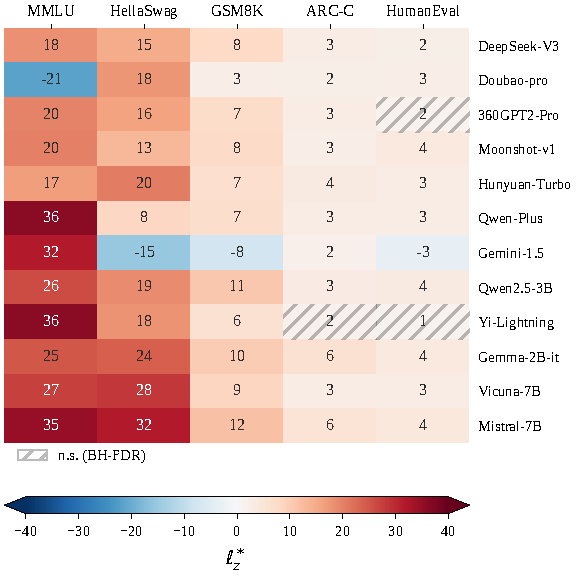
\includegraphics[width=\columnwidth]{fig_4_model_heatmap.pdf}
  \caption{$\ell_z^*$ heatmap for 12 leaderboard models across five benchmarks. 57/60 cells exceed $|\ell_z^*| > 1.96$, indicating pervasive IRT assumption violations even absent contamination. Details in Appendix~\ref{app:leaderboard_aberrance}.}
  \label{fig:leaderboard_heatmap}
\end{figure}

\subsection{Ability-Dependent Non-Monotonic Dose-Response}
\label{sec:inverted_u}

As an exploratory observation, the free-$\theta$ dose-response is non-monotonic for Qwen.
Figure~\ref{fig:dose_response} plots the dose-response trajectory, combining the single-seed 5\% estimate (hollow marker) with multi-seed means at 15\%/25\%/50\% ($|d|$: $4.15 \to 5.36 \to 7.44 \to 5.08$), showing signal peaking at 25\% before declining; inter-seed variance at 50\% is high (CV${=}$60\%, range $[1.90, 7.91]$).
This non-monotonicity is a $\theta$-estimation artifact: fixed-$\theta$ eliminates the inverted-U ($|d|{=}12.32$ at 50\%, CV reduced to 19\%).
Llama's flat trajectory ($|d|{\approx}2.3$--$2.8$) is consistent with its near-zero baseline $\ell_z^*$: the divergence is fully explained by baseline ability differences.
Simulation corroborates: two-sided testing achieves ${>}$93\% power at all levels on MMLU (Appendix~\ref{app:simulation}).
These results demonstrate that non-monotonic dose-response is not a fundamental limitation of person-fit statistics but a predictable consequence of free-$\theta$ estimation in high-ability models, and that $\theta$-anchoring provides a principled correction.
